%%%%%%%%%%%%%%%%%%%%%%%%%%%%%% -*- Mode: Latex -*- %%%%%%%%%%%%%%%%%%%%%%%%%%%%
%% textemplate.tex -- Thesis Proposal
%% Author          : Burt Leung
%% Created On      : Mon Oct 28 2004
%% Last Modified By: 
%% Last Modified On: Mon Oct 28 2004
%% RCS: $Id$
%%%%%%%%%%%%%%%%%%%%%%%%%%%%%%%%%%%%%%%%%%%%%%%%%%%%%%%%%%%%%%%%%%%%%%%%%%%%%%%
%%   Copyright (C) 2004 Burt Leung
%%%%%%%%%%%%%%%%%%%%%%%%%%%%%%%%%%%%%%%%%%%%%%%%%%%%%%%%%%%%%%%%%%%%%%%%%%%%%%%
%% 


\documentclass[11pt,twocolumn]{article} 
\input{/export/home/csdl/tex/psfig/psfig}
\usepackage{/export/home/csdl/tex/icse2003/latex8}
\usepackage{times}
%% A verbatim-like environment which allows font changes
%%\usepackage{alltt}
%% New LaTeX2e graphics support
\usepackage[final]{graphicx}
% uncomment the % away on next line to produce the final camera-ready version
% and uncomment the \thispagestyle{empty} following \maketitle
\pagestyle{empty}

\begin{document}

\title{Improving The Development Process By Examining Software Defects}


\author{\protect\begin{tabular}{ccc}
Burt Leung
\end{tabular}\\
\em  Collaborative Software Development Laboratory \\
\em  Department of Information and Computer Sciences \\
\em  University of Hawai'i \\
\em  Honolulu, HI 96822 \\
\em  bleung@hawaii.edu}
\maketitle
\thispagestyle{empty}

\begin{abstract}  % 200 words

Software defects (SD) are a natural but undesirable by-product of developing software. If there are too many defects then developers can end up spending all their time fixing SD rather than engineering software. 

Currently, there are two primary methods to address SD. One way is by means of the Software Review process (SR) in which a software development artifact is evaluated, usually by members of the development team. The other way is Defect Tracking (DT) where users of the software will identify bugs and improvement opportunities and enter them into an issue management system.

Each of the two approaches is very different in getting defect data. It is entirely possible that either presents information about different kinds of defects that the other does not make obvious. I claim that: (a) Software reviews are more likely to uncover software defects that impact maintenance and standards (b) defect tracking is more likely to collect software defects that have to do with class level design, communication between objects, timing and serialization, the build process, and relationships between objects (c) the software review process can be improved by getting feedback from defect tracking data (d) The results of a software review can feed forward into the defect tracking system.

There are many studies that focus on either SR or DT in one way or another. However, there has not been a concrete strategy that has emerged from these past studies on how to improve the software development process by using feedback from analyzing defect data of both SR and DT.

My approach in this study will be to gather SD data from both SR and DT and analyze how the SR process can be improved by feedback gotten from DT or vice-versa. I believe that this research will reveal new opportunities to improve the software development process through integrated and in-process analysis of SR and DT defect streams.

To implement this evaluation I will collect data from SR and DT performed by the Hackystat development team. Once the data is collected I will classify the defects using the Orthogonal Defect Classification (ODC) and then identify possible process improvements which I will propose to the Hackystat developers. Upon their approval the proposed strategies will be put into practice.

The efficacy of the experiment will be determined by monitoring the defect stream for desirable changes. A qualitative evaluation will also be performed by distributing a questionnaire to the Hackystat developers on the merits of the proposed process improvements and the results of putting them into practice.

In the beginning of the Spring 2005 semester I will have a sensor for the Jira Issue management system implemented with some preliminary sensor data collected. In order to collect defect data from SR I will utilize the Jupiter tool and sensor which is a plug-in to the Eclipse IDE that facilitates SR. I will continue to collect more SD data as well as implement the analyses during January and February. March will be the month to wrap up my study, conduct the qualitative evaluations and write up my thesis report.

\end{abstract}

\Section{Introduction}

(Introduce the concept of software defects)

(Introduce the concept of defect tracking systems)

(Introduce the concept of software reviews)

In this study I will use the Orthogonal Defect Classification scheme (ODC). It is a thorough method of classifying all aspects of a defect from the time it is discovered to the time it is resolved. In order to do this ODC specifies a number of attributes that describe a given defect. The attributes of ODC fall into two categories, openers and closers. 
      
The opener attributes are those that can be assessed when the defect is found. These include (a) the activity that was being performed at the time the defect was discovered (b) the condition or trigger that produced the defect (c) the type of impact that the defect has. 
      
The closer attributes are those that can be classified when a fix for the defect is known. These include (a) the target type of the fix (b) the correction type (c) the defect qualifier (d) the age of the defect (e) the source of the defect.

(Introduce proposed idea of using DT and SR to feedback to each other)

\label{sec:intro}

\Section{Related Work}

The main cause of software product failures is due to SD \cite{sullivan91software}. There are many different types of SD and they range in severity as well.
      
In the current literature, SR is documented as a highly effective process for determining SD. It is able to efficiently find SD in source code and therefore can save time and money. One of the current weaknesses of SR is determining which section of source code should be inspected. While there are numerous studies that testify to its cost effectiveness it is also true that it is not known how many defects are originally in a product and where to look for the defects \cite{porter96review}. 
      
To address this weakness the focus of current research is to improve upon the SR process. It has been demonstrated that altering factors such as the people involved, the code units, and review techniques can influence the effectiveness of the SR \cite{porter98understanding}. 
      
Current review practices for SR are usually conducted by having members of the development team review the source code together and determine SD that must be addressed. Sometimes an aid such as checklists are used to help direct which source code should be reviewed. A newer technique involves perspective-based reading (PBR) in which reviewers assume a particular role while doing the critique. PBR has been found to have a 58% cost per defect improvement over checklist-based reading \cite{laitenberger00experimental}.
      
DT is done by an issue management system which is able to record an SD and then track changes and updates to its condition. It is especially good at bringing together users and developers of the system. With the DT system a user of the software product can report an SD anonymously and the personnel most qualified to respond to it can do so \cite{development-bug}. 
      
It has been realized that the data tracked in DT systems can be analyzed and used to improve software quality \cite{fredericks-using}. Current analyses techniques involve generating a baseline and then performing statistical and root cause analysis. The feedback given from these analyses gives the developers a deeper understanding about the software product and the development process.

\label{sec:related}

\Section{Software Tools}

In order to collect defect data from a DTS and SR I will utilize the DT and SR tools that CSDL currently uses. In order to facilitate classifying each defect that I will examine I have designed a database with a website front for data-entry.
      
In order to allow for complex queries against the collected data I engineered the database and its tables using SQL Server 2000. Each record is meant to contain ODC attributes for each defect that I examine. Each record will contain a field for each ODC attribute. I also added fields to capture the defect�s summary, workspaces, reporter, assignee, date discovered, date resolved, and severity. Most importantly I have a field that describes the tool that collected or generated the SD, either Jira or Jupiter. This will enable me to distinguish data from the two tools.
      
In order to enter the data into the database I created a web-application front-end. It allows for registration of a new defect classification, viewing and editing of existing classification entries, and generating charts from the data. 

\begin{figure*}[ht]
  \centering
  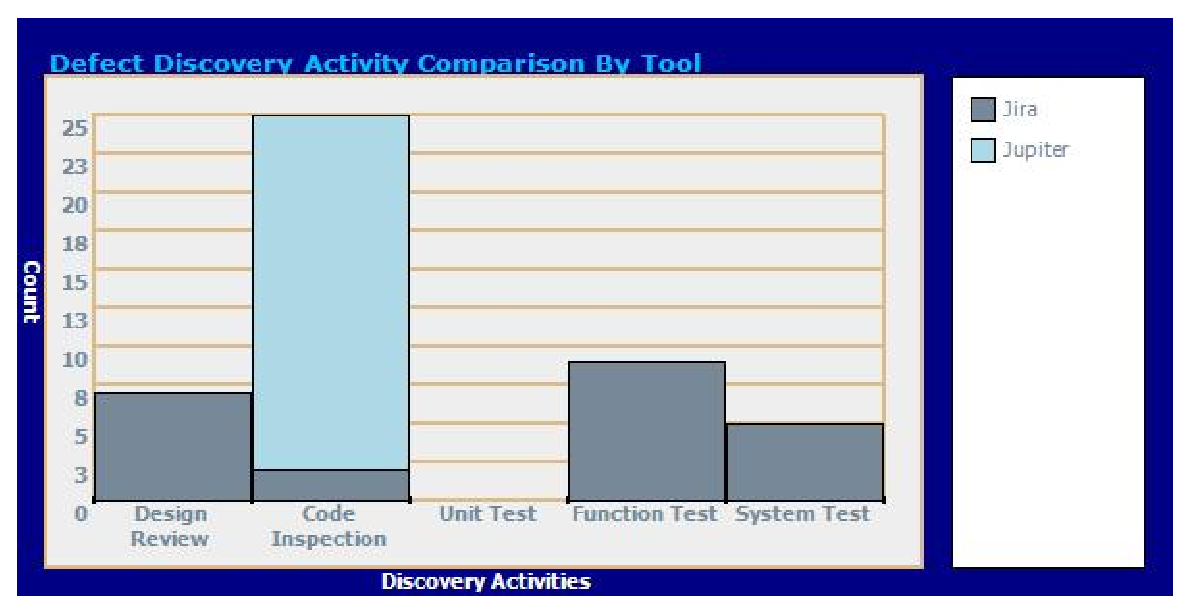
\includegraphics[width=0.75\textwidth]{stackedchart.eps}
  \caption{A stacked chart from my pilot study results}
  \label{fig:architecture}
\end{figure*}

I decided to go with a stacked chart representation of the data. It has the advantage of showing the total count of defects for a specific attribute and one can also compare the distribution of the tool type within each bar itself. With the graphs it is easy to compare the distribution of defects according to the tool used to collect or generate the SD.
      
Jira is the issue management system that is used by CSDL. It is developed by Atlassian.com and it is web based and very customizable. It allows for users to define their own issue templates specific to their organization. 
      
For the purposes of my study I will use Jira by periodically looking over the SD entries collected and then populating my database with an ODC record for each one. Coincidentally I have just implemented a Hackystat sensor (see http://www.hackystat.org) which automatically collects issue data from Jira. Unfortunately there is no way to automatically classify each defect which is why this portion of my study must be done manually.
      
Jupiter is an existing tool and extension to the Eclipse integrated development environment created by Takuya Yamashita. It facilitates SR by supporting three phases of the process. In the first phase, developers enter their personal criticisms individually. In the second phase the entire team looks over all the issues together and decides on the validity of each criticism as a group. In the final phase the author of the source code will rework each SD determined to be valid.

\label{sec:system}

\Section{Evaluation Methodology}

A pilot study was initially done in order to form the basis of my hypotheses. I examined and classified 23 defects in Jira and then classified 23 defects generated by Jupiter. The results were very interesting. The classification scheme used was ODC. 
      
In the charts that I generated from the data I found that Jira data was more likely to capture defects impacting areas such as reliability and capability while the Jupiter data was more likely to capture defects impacting source code maintenance and coding standards. The Jira data also covered a broader range of defect types, all very important to the quality of the software product. Therefore, from the pilot study I found that merely doing code reviews is not enough to capture all SD. Both Jira and Jupiter give defect data that each individual tool would not have caught alone. 
      
The pilot study yielded some interesting results that helped form my claims. In order to test them a more in-depth study needs to be conducted from a larger sample size of defect data. In the following semester I will aim re-do the pilot study on a larger scale. I hope to collect about 200 defects from each type of tool, Jira and Jupiter.

\subsection{Evaluating claim 1: Software reviews are more likely to uncover software defects that impact maintenance and standards.}
      
It is not surprising that SR would yield defects with a code-level scope. Things like the naming of variables and a better way to implement a method are common examples of SD derived from a code review. Reviewers commonly compare code to the development team�s coding styles and standards to generate criticisms. They also look for code that could be refactored into something simpler and easier to maintain.
      
In order to evaluate this claim I will once again take a look at the defect classifications made from Jupiter data. Then I will validate whether or not the same results from my pilot study still hold.

\subsection{Evaluating claim 2: Defect tracking is more likely to collect software defects that have to do with class level design, communication between objects, timing and serialization, the build process, and relationships between objects.}
      
DT is more likely to collect defect data that deal with issues not immediately obvious from a code inspection. One of the biggest reasons behind this is because the trigger that exposes a defect reported to Jira can be very diverse. For example, it could have been noticed by exercising a particular module, or it could have been made visible by a malfunction in the user interface, etc. On the other hand the SR only has one trigger and that is the inspection process itself.

In order to evaluate the second claim I will take a look at the defect classifications that I did for the Jira data.

\subsection{Evaluating claim 3: The software review process can be improved by getting feedback from defect tracking data.}
      
For a period of a month I will examine each week�s SD collected in Jira and determine one to a few defects of concern (DOC). These are to be SD that are of high severity and could cause critical problems with the software product�s capability or reliability. I will then look at the trigger activities that lead to each DOC. These triggers will guide the next software review.
      
For example, if Jira captures a DOC and the trigger was from a failed system level function then the next SR needs to focus on the cause of this problem. Since the trigger was a system level occurrence the SR might need to look at the class level design instead of focusing on the code within a couple of specific classes.
      
With each subsequent week, if the DOC type has changed or decreased in number then this can be interpreted as an improvement on the process. This would mean that the feedback provided by Jira into the SR process is a success.
      
A subjective evaluation will be applied here as well. The developers involved with the SR and DT in CSDL will be given a questionnaire to fill out on their opinion about the effectiveness of my intervention.

\subsection{Evaluating claim 4: The results of a software review can feed forward into the defect tracking system.}
      
Each week for the month long experiment I will take note of SD generated from Jupiter and determine if they deserve to be tracked or not. I will also take note of SD that affect or relate to existing defects tracked in Jira and update them according.
      
If I am unable to find any defects that relate to existing defects in Jira or any that qualify as new entries into Jira then I could consider this claim as false. However I expect that a feed forward process will prove successful.
      
As with the previous claim a subject evaluation in the form of a questionnaire will be given out. Those involved with the development process will give their opinion about the effectiveness of the feed forward process.

\label{sec:evaluation}

\Section{Results}

(Pending)

\label{sec:results}

\Section{Contributions and future directions}

(Pending)

\label{sec:contributions}

\Section{Acknowledgements}

(Pending)

\label{sec:acknowledgements}

\bibliographystyle{/export/home/csdl/tex/icse2003/latex8}
\bibliography{/export/home/csdl/techreports/04-19/textemplate,/export/home/csdl/bib/csdl-trs,/export/home/csdl/bib/hackystat,/export/home/csdl/bib/psp}
\end{document}







